% ============================================================================
% CHƯƠNG 1: TỔNG QUAN (INTRODUCTION)
% ============================================================================

\chapter{TỔNG QUAN}

\section{Đặt vấn đề}

Trong kỷ nguyên số hóa hiện nay, ngành công nghiệp trò chơi điện tử (gaming) đang chứng kiến sự phát triển bùng nổ với quy mô thị trường toàn cầu đạt hàng trăm tỷ USD. Cùng với sự phát triển này là lượng nội dung đánh giá, thảo luận về game trên các nền tảng mạng xã hội tăng theo cấp số nhân. Các nền tảng như \textbf{Reddit} (với các subreddit gaming lớn như r/gaming, r/Games, r/pcgaming), \textbf{Steam}, \textbf{Metacritic}, và \textbf{Twitter} mỗi ngày tiếp nhận hàng triệu bài viết, bình luận từ cộng đồng người chơi.

Việc phân tích cảm xúc (sentiment analysis) từ khối lượng dữ liệu khổng lồ này mang lại giá trị to lớn cho nhiều đối tượng: các nhà phát triển game có thể nắm bắt phản hồi cộng đồng để cải thiện sản phẩm, nhà phân phối có thể đánh giá xu hướng thị trường, và người tiêu dùng có thể tham khảo đánh giá trước khi mua game. Tuy nhiên, việc áp dụng các phương pháp sentiment analysis truyền thống vào lĩnh vực gaming gặp phải ba thách thức đặc thù:

\subsection{Thách thức 1: Đặc trưng ngôn ngữ gaming phức tạp}

Ngôn ngữ được sử dụng trong cộng đồng game thủ mang những đặc điểm chuyên biệt, khác xa với ngôn ngữ phổ thông, tạo ra rào cản lớn cho các phương pháp phân tích cảm xúc truyền thống. Đầu tiên là sự xuất hiện dày đặc của các thuật ngữ kỹ thuật (technical jargon) như \textbf{"FPS drop"}, \textbf{"input lag"} hay \textbf{"hitbox"}; đòi hỏi mô hình phải hiểu được ngữ nghĩa chuyên ngành thay vì nghĩa đen thông thường. Bên cạnh đó, hệ thống tiếng lóng (slang) và từ viết tắt như \textbf{"P2W"} (pay-to-win) hay \textbf{"GOTY"} (Game of the Year) phát triển mạnh mẽ và thay đổi liên tục theo xu hướng. Khó khăn hơn cả là tính đa nghĩa theo ngữ cảnh (contextual polysemy) và sự phổ biến của lối nói châm biếm (sarcasm). Một từ ngữ mang sắc thái tích cực như \textbf{"masterpiece"} hoặc \textbf{"optimized"} hoàn toàn có thể được sử dụng để biểu đạt sự mỉa mai tiêu cực khi đi kèm với các bối cảnh lỗi game, khiến việc xác định đúng cảm xúc trở nên vô cùng phức tạp.

\subsection{Thách thức 2: Chi phí gán nhãn thủ công cao}

Việc xây dựng bộ dữ liệu huấn luyện chất lượng cao cho mô hình học có giám sát (Supervised Learning) đối mặt với bài toán nan giải về chi phí và khả năng mở rộng. Quá trình gán nhãn thủ công không chỉ đòi hỏi nguồn lực tài chính lớn để thuê chuyên gia có kiến thức nền tảng về game, mà còn tiêu tốn lượng thời gian đáng kể để xử lý hàng chục nghìn bài viết. Hơn nữa, tính nhất quán của dữ liệu thường không được đảm bảo do sự khác biệt trong quan điểm chủ quan của từng người gán nhãn (annotator), đặc biệt đối với các nội dung mang tính subjective. Đặc biệt, với tốc độ sinh dữ liệu khổng lồ hàng ngày trên các nền tảng mạng xã hội, phương pháp thủ công trở nên bất khả thi trong việc đáp ứng nhu cầu cập nhật dữ liệu liên tục ở quy mô lớn.

\subsection{Thách thức 3: Mất cân bằng dữ liệu tự nhiên}

Dữ liệu thực tế trong lĩnh vực gaming thường tồn tại sự mất cân bằng phân phối nghiêm trọng (class imbalance). Do tâm lý hành vi người dùng thường có xu hướng chia sẻ nhiều hơn khi hài lòng, dữ liệu gaming thường gặp hiện tượng "positive bias" với nhãn \textbf{Positive} chiếm đa số (thường dao động 40-50\%), trong khi các đánh giá \textbf{Negative} (Tiêu cực)—nguồn thông tin quan trọng nhất cho nhà phát triển—lại chỉ chiếm tỷ lệ thiểu số (15-20\%). Ngoài ra, lớp \textbf{Neutral} mang tính chất thảo luận hoặc hỏi đáp thường xuyên bị chồng lấn (overlapping) ranh giới với hai lớp còn lại. Sự mất cân bằng này khiến các mô hình học máy truyền thống dễ bị thiên kiến (bias) về phía lớp đa số để tối ưu hóa hàm mất mát, dẫn đến việc bỏ qua hoặc nhận diện kém các đặc trưng quan trọng của lớp thiểu số \cite{lin2017focal}.

% ----------------------------------------------------------------------------
\section{Mục tiêu nghiên cứu}

Nghiên cứu này đặt ra ba mục tiêu chính nhằm giải quyết các thách thức đã nêu:

\subsection{Mục tiêu 1: Xây dựng hệ thống Weak Supervision cho Gaming Domain}

Mục tiêu đầu tiên là phát triển một hệ thống tự động gán nhãn cảm xúc cho nội dung gaming trên Reddit, tận dụng các tín hiệu cộng đồng (community signals) để thay thế quy trình gán nhãn thủ công tốn kém. Quá trình này bao gồm ba bước chính:

Đầu tiên, \textbf{thu thập dữ liệu} được thực hiện bằng cách crawl bài viết từ 6 subreddit gaming lớn bao gồm: r/gaming, r/Games, r/pcgaming, r/gamernews, r/gamedev, và r/indiegaming.

Tiếp theo, đề tài \textbf{thiết kế chiến lược 8-Signal}, kết hợp 8 loại tín hiệu với trọng số khác nhau để suy luận nhãn:
\textbf{Awards} (trọng số 4.0 - tín hiệu mạnh nhất),
\textbf{Comments Count} (3.0 - mức độ engagement),
\textbf{Upvote Ratio} (2.5 - sự đồng thuận),
\textbf{Post Score} (2.0 - độ phổ biến),
\textbf{Gaming Text Features} (1.8-3.0 - từ vựng đặc thù),
\textbf{Sarcasm Detection} (cơ chế đảo chiều sentiment),
\textbf{Flair Analysis} (2.0-3.5 - phân loại từ nhãn bài viết), và
\textbf{Top Comments} (2.0-2.5 - phân tích phản hồi cộng đồng).

Cuối cùng, hệ thống sử dụng \textbf{Weighted Voting Mechanism} để tổng hợp các tín hiệu trên với trọng số động (dynamic weighting từ 1.8 đến 3.5) kèm theo điểm tin cậy (confidence scoring) nhằm tạo ra các nhãn yếu (weak labels) chất lượng cao. Hiệu quả của phương pháp sẽ được đánh giá thông qua việc so sánh Accuracy, F1-score và thời gian huấn luyện với phương pháp Supervised Learning truyền thống.

\subsection{Mục tiêu 2: Giải quyết bài toán Class Imbalance}

Để khắc phục hiện tượng mất cân bằng dữ liệu nghiêm trọng trong lĩnh vực gaming, đề tài nghiên cứu và so sánh hai nhóm phương pháp chính:

\subsubsection{Phương pháp Algorithm-Level (Focal Loss và Class Weighting)}

Đối với hướng tiếp cận ở mức thuật toán, đề tài tập trung vào Focal Loss, một kỹ thuật giúp mô hình tập trung vào các mẫu khó phân loại. Công thức toán học được định nghĩa như sau:

\begin{equation}
    FL(p_t) = -\alpha_t (1 - p_t)^{\gamma} \log(p_t)
\end{equation}

Trong đó, $p_t$ là xác suất dự đoán đúng của mẫu. Tham số $\alpha$ đóng vai trò trọng số cân bằng lớp, trong khi $\gamma$ là tham số tập trung (focusing parameter) giúp giảm trọng số của các mẫu dễ (easy examples) thông qua hệ số điều chỉnh $(1-p_t)^{\gamma}$.

Bên cạnh đó, phương pháp Class Weighting cũng được áp dụng để tích hợp trọng số vào hàm CrossEntropyLoss, trong đó lớp thiểu số sẽ nhận trọng số cao hơn dựa trên công thức:
\begin{equation}
    w_j = \frac{N}{K \cdot n_j}
\end{equation}
Với $N$ là tổng số mẫu, $K=3$ là số lượng lớp, và $n_j$ là số mẫu của lớp $j$. Ưu điểm của phương pháp này là đơn giản hơn Focal Loss do không cần tinh chỉnh các siêu tham số $\alpha, \gamma$.

\subsubsection{Phương pháp Data-Level (Undersampling)}

Ở mức dữ liệu, phương pháp \textbf{Undersampling} được sử dụng làm cơ sở so sánh (baseline). Kỹ thuật này giảm số lượng mẫu của lớp đa số xuống mức cân bằng với lớp thiểu số (từ 21,821 xuống 12,093 mẫu). Mặc dù đảm bảo sự cân bằng hoàn toàn, phương pháp này phải đánh đổi bằng việc mất đi một lượng lớn dữ liệu huấn luyện ($\sim$9,728 mẫu).

\subsection{Mục tiêu 3: So sánh định lượng các phương pháp}

Mục tiêu cuối cùng là xây dựng một pipeline gồm 4 giai đoạn (Stages) để thực hiện so sánh toàn diện giữa Weak Supervision và các chiến lược Supervised Learning:

\begin{figure}[H]
    \centering
    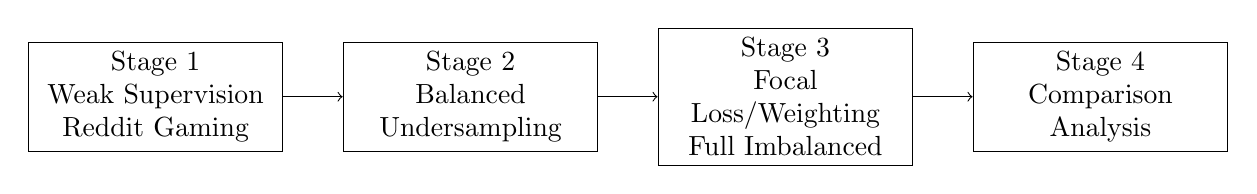
\begin{tikzpicture}[node distance=1cm]
        \node (stage1) [rectangle, draw, text width=3cm, align=center] {Stage 1\\Weak Supervision\\Reddit Gaming};
        \node (stage2) [rectangle, draw, text width=3cm, align=center, right of=stage1, xshift=3cm] {Stage 2\\Balanced\\Undersampling};
        \node (stage3) [rectangle, draw, text width=3cm, align=center, right of=stage2, xshift=3cm] {Stage 3\\Focal Loss/Weighting\\Full Imbalanced};
        \node (stage4) [rectangle, draw, text width=3cm, align=center, right of=stage3, xshift=3cm] {Stage 4\\Comparison\\Analysis};
        
        \draw [->] (stage1) -- (stage2);
        \draw [->] (stage2) -- (stage3);
        \draw [->] (stage3) -- (stage4);
    \end{tikzpicture}
    \caption{Pipeline 4 stages so sánh Weak Supervision và Supervised Learning}
\end{figure}

Các phương pháp sẽ được đánh giá đa chiều dựa trên 5 tiêu chí: (1) \textbf{Accuracy \& F1-Score} (hiệu suất phân loại), (2) \textbf{Training Time} (tốc độ huấn luyện), (3) \textbf{Dataset Efficiency} (mức độ tận dụng dữ liệu), (4) \textbf{Labeling Cost} (chi phí gán nhãn), và (5) \textbf{Per-Class Performance} (hiệu quả trên từng lớp cụ thể: Negative, Neutral, Positive).


% ----------------------------------------------------------------------------
\section{Đối tượng và phạm vi nghiên cứu}

\subsection{Nguồn dữ liệu nghiên cứu}

\subsubsection{Dữ liệu Weak Supervision (Stage 1)}

Để xây dựng bộ dữ liệu huấn luyện cho mô hình Weak Supervision, nghiên cứu tập trung thu thập dữ liệu từ \textbf{Reddit} - nền tảng thảo luận lớn nhất thế giới về gaming. Cụ thể, dữ liệu được crawl từ 6 subreddit tiêu biểu bao gồm: \textbf{r/gaming} ($\sim$35M thành viên), \textbf{r/Games} ($\sim$3M thành viên - tập trung vào thảo luận chất lượng cao), \textbf{r/pcgaming} ($\sim$2.5M thành viên), \textbf{r/gamernews}, \textbf{r/gamedev}, và \textbf{r/indiegaming}.

Các subreddit này được lựa chọn dựa trên các tiêu chí khắt khe nhằm đảm bảo chất lượng dữ liệu: số lượng thành viên đông đảo ($>$100K), tần suất đăng bài cao ($>$100 bài/ngày), tỷ lệ spam thấp ($<$5\%) và mức độ tương tác tốt (tỷ lệ upvote trung bình $>$0.7). Nội dung thảo luận bao phủ đa dạng các chủ đề từ tin tức, review, phát triển game đến trải nghiệm người chơi.

Quá trình thu thập được thực hiện thông qua thư viện \textbf{PRAW} (Python Reddit API Wrapper), giới hạn trong các bài đăng thuộc tháng 11/2025. Các từ khóa tìm kiếm (keywords) được sử dụng bao gồm: "game", "gaming", "gameplay", "review", "experience", "bug", "issue", "performance", "story", và "fun".

\subsubsection{Dữ liệu Supervised Learning (Stage 2, 3)}

Đối với giai đoạn huấn luyện có giám sát, nghiên cứu sử dụng bộ dữ liệu chuẩn \textbf{"Reddit Gaming Comments with Sentiments"} từ Kaggle\footnote{\url{https://www.kaggle.com/datasets/sainitishmitta04/23k-reddit-gaming-comments-with-sentiments-dataset}}. Bộ dữ liệu này bao gồm \textbf{21,821} bình luận game (game reviews) được tổng hợp từ Steam và Reddit, đã qua quá trình gán nhãn thủ công.

Một đặc điểm quan trọng của bộ dữ liệu này là sự mất cân bằng tự nhiên (Natural Imbalance) trong phân phối nhãn: lớp \textbf{Positive} chiếm đa số ($\sim$44.8\%), theo sau là lớp \textbf{Neutral} ($\sim$35.7\%), trong khi lớp \textbf{Negative} chỉ chiếm tỷ lệ thiểu số ($\sim$18.5\%), tạo ra tỷ lệ mất cân bằng khoảng 2.43:1 giữa lớp Positive và Negative. Dữ liệu bao gồm hai trường thông tin chính là nội dung văn bản (\texttt{comment}) và nhãn cảm xúc (\texttt{sentiment}).

Quy trình xử lý dữ liệu được chia làm hai hướng phục vụ cho các giai đoạn khác nhau: Tại \textbf{Stage 2}, kỹ thuật Undersampling được áp dụng để cân bằng số lượng mẫu, giảm kích thước dữ liệu xuống còn \textbf{12,093} mẫu. Ngược lại, ở \textbf{Stage 3}, toàn bộ \textbf{21,821} mẫu dữ liệu gốc được giữ nguyên để nghiên cứu hiệu quả của các phương pháp xử lý mất cân bằng dữ liệu.

\subsection{Mô hình nghiên cứu}

Nghiên cứu lựa chọn mô hình nền tảng (Base Model) là \\
\texttt{cardiffnlp/twitter-roberta-base-sentiment-latest} \cite{liu2019roberta}. Quyết định này dựa trên bốn ưu điểm vượt trội của kiến trúc RoBERTa-Twitter:

Thứ nhất, mô hình được \textbf{tối ưu hóa cho văn bản mạng xã hội} nhờ quá trình pre-training trên 124 triệu tweets. Điều này giúp mô hình xử lý hiệu quả các đặc trưng ngôn ngữ không chính thức như emoji, tiếng lóng (slang), và các ngữ cảnh ngắn ($<$512 tokens) thường gặp trong bình luận game.

Thứ hai, mô hình sở hữu \textbf{kiến trúc mạnh mẽ} với 12 lớp Transformer, 125 triệu tham số và bộ từ vựng (vocabulary) lên đến 50K tokens, bao quát tốt các thuật ngữ chuyên ngành gaming.

Thứ ba, RoBERTa-Twitter đã chứng minh \textbf{hiệu năng vượt trội} khi đạt kết quả SOTA (State-of-the-Art) trên bộ dữ liệu SemEval-2017 Sentiment Analysis và độ chính xác xấp xỉ 92\% trên các tác vụ phân tích cảm xúc Twitter, cho thấy khả năng tổng quát hóa tốt sang miền dữ liệu gaming.

Cuối cùng, khả năng \textbf{Transfer Learning hiệu quả} cho phép tinh chỉnh (fine-tune) mô hình nhanh chóng mà không cần huấn luyện lại từ đầu, đồng thời giảm thiểu hiện tượng overfitting nhờ vào nền tảng pre-training vững chắc.

\subsection{Phạm vi bài toán}

\subsubsection{Loại bài toán và Output Classes}

Đề tài tập trung giải quyết bài toán \textbf{Multi-class Classification} với 3 lớp cảm xúc đầu ra:

\begin{itemize}
    \item \textbf{Positive (Tích cực):} Bao gồm các đánh giá tốt, lời khen ngợi hoặc khuyến nghị chơi game. Ví dụ: "This game is a masterpiece!", "Best GOTY contender".
    \item \textbf{Neutral (Trung lập):} Bao gồm các thảo luận khách quan, câu hỏi hoặc chia sẻ thông tin thuần túy. Ví dụ: "What's your opinion on this game?", "Graphics are good but story is meh".
    \item \textbf{Negative (Tiêu cực):} Bao gồm các phản hồi tiêu cực, báo cáo lỗi (bug report) hoặc phàn nàn gay gắt (rant). Ví dụ: "Broken mess, avoid this!", "P2W garbage".
\end{itemize}

\subsubsection{Metrics đánh giá và Giới hạn phạm vi}

Để đánh giá toàn diện hiệu quả của mô hình, nghiên cứu sử dụng tập hợp các chỉ số đo lường bao gồm: \textbf{Accuracy} (tỷ lệ phân loại đúng tổng thể), \textbf{F1-Score Weighted} (trọng số theo kích thước lớp), \textbf{F1-Score Macro} (trung bình không trọng số), cùng với \textbf{Precision/Recall} cho từng lớp và \textbf{Confusion Matrix} để phân tích chi tiết các trường hợp phân loại sai. Bên cạnh đó, \textbf{Training Time} cũng được ghi nhận để so sánh chi phí tính toán.

Nghiên cứu giới hạn phạm vi trong phân tích cảm xúc dựa trên văn bản (Text-based sentiment) từ các nguồn reviews và comments. Các hướng tiếp cận đa phương thức (Multi-modal) kết hợp hình ảnh, phân tích cảm xúc theo khía cạnh (Aspect-based), hay phân tích cảm xúc chi tiết (Emotion analysis như vui, giận, sợ hãi...) nằm ngoài phạm vi của đề tài này.

% ----------------------------------------------------------------------------
\section{Đóng góp của đề tài}

Nghiên cứu mang lại những đóng góp quan trọng cho lĩnh vực Phân tích cảm xúc trong miền dữ liệu Gaming, cụ thể trên các phương diện sau:

\subsection{Đóng góp 1: Chiến lược 8-Signal Weak Supervision cho Gaming}

\textbf{Tính mới:} Đề tài đề xuất hệ thống gán nhãn yếu (weak labeling) đầu tiên được tối ưu hóa riêng cho miền dữ liệu gaming, kết hợp 8 loại tín hiệu cộng đồng với cơ chế trọng số động \cite{ratner2017snorkel}. Hệ thống tín hiệu được phân thành ba nhóm chính:

Đầu tiên là nhóm \textbf{tín hiệu siêu dữ liệu (Metadata Signals)}, đóng vai trò chỉ báo định lượng mạnh mẽ. Trong đó, \textbf{Awards} (Gold, Platinum...) được xem là tín hiệu cao nhất với trọng số 4.0 do gắn liền với chi phí thực tế. Các chỉ số khác bao gồm \textbf{Comments Count} (trọng số 3.0) phản ánh mức độ tương tác, \textbf{Upvote Ratio} (trọng số 2.5) thể hiện sự đồng thuận, và \textbf{Post Score} (trọng số 2.0) đại diện cho độ phổ biến của bài viết.

Tiếp theo là nhóm \textbf{tín hiệu nội dung (Content Signals)}, tập trung khai thác đặc trưng văn bản. Hệ thống phân tích \textbf{Gaming Text Features} (trọng số 1.8-3.0) dựa trên các từ khóa chuyên ngành (ví dụ: "masterpiece" là tích cực, "broken mess" là tiêu cực). Đặc biệt, cơ chế \textbf{Sarcasm Detection} được tích hợp để xử lý các trường hợp châm biếm (như tag "/s" hoặc ngữ cảnh mâu thuẫn), cho phép đảo chiều nhãn cảm xúc chính xác.

Cuối cùng là nhóm \textbf{tín hiệu ngữ cảnh (Context Signals)}, bao gồm \textbf{Flair Analysis} (trọng số 2.0-3.5) để tận dụng nhãn phân loại có sẵn của bài viết (ví dụ: flair "Bug" mang nghĩa tiêu cực), và \textbf{Top Comments Sentiment} (trọng số 2.0-2.5) nhằm phân tích phản hồi từ cộng đồng thông qua 3 bình luận nổi bật nhất.

Các tín hiệu trên được tổng hợp thông qua cơ chế Weighted Voting Mechanism để tính toán độ tin cậy (Confidence):

\begin{equation}
    \text{Confidence} = \frac{\sum_{i=1}^{8} w_i \cdot \mathbb{1}(\text{signal}_i = \text{label})}{\sum_{i=1}^{8} w_i}
\end{equation}

Trong đó $w_i$ là trọng số của tín hiệu thứ $i$ và hàm chỉ thị $\mathbb{1}$ nhận giá trị 1 nếu tín hiệu đồng thuận với nhãn dự đoán. Nhãn cuối cùng chỉ được chấp nhận nếu độ tin cậy vượt ngưỡng 0.6.

\subsection{Đóng góp 2: Phân tích sâu Class Imbalance với Focal Loss và Class Weighting}

\textbf{Tính mới:} Đề tài thực hiện nghiên cứu chuyên sâu và so sánh hai phương pháp algorithm-level để giải quyết vấn đề mất cân bằng dữ liệu trong phân tích cảm xúc gaming: Focal Loss và Class Weighting.
\\
Về mặt kỹ thuật, Focal Loss được hiện thực hóa dựa trên công thức:
\begin{equation}
    FL(p_t) = -\alpha_t (1 - p_t)^{\gamma} \log(p_t)
\end{equation}

Quy trình tính toán bắt đầu bằng việc chuyển đổi logits thành xác suất qua hàm softmax, sau đó xác định xác suất dự đoán đúng $p_t$ cho nhãn thực tế. Trọng số focal (focal weight) được tính toán bằng $(1 - p_t)^{\gamma}$ và áp dụng vào hàm loss Cross Entropy tiêu chuẩn. Các siêu tham số được tinh chỉnh cụ thể: \textbf{Alpha ($\alpha$) = 0.25} giúp cân bằng trọng số giữa lớp Positive và Negative, trong khi \textbf{Gamma ($\gamma$) = 2.0} đóng vai trò tham số tập trung, giúp giảm trọng số của các mẫu dễ phân loại và buộc mô hình học kỹ hơn các mẫu khó.
\\
Song song với Focal Loss, đề tài cũng triển khai phương pháp Class Weighting sử dụng trọng số nghịch đảo logarit:
\begin{equation}
    w_j = \frac{1}{\ln(1 + n_j)}, \quad \text{chuẩn hóa: } w_j' = \frac{w_j}{\sum_{k=1}^{K} w_k}
\end{equation}

Trọng số này được tích hợp trực tiếp vào Weighted Cross-Entropy Loss, trong đó lớp thiểu số nhận trọng số cao hơn để cân bằng đóng góp vào gradient. Ưu điểm của Class Weighting là tính đơn giản trong triển khai (không cần tinh chỉnh $\alpha, \gamma$) và ổn định trong quá trình huấn luyện nhờ logarit giảm chênh lệch trọng số quá lớn.


\subsection{Đóng góp 3: Gaming-Specific Lexicon}

\textbf{Tính mới:} Đề tài xây dựng và chuẩn hóa một bộ từ điển cảm xúc chuyên biệt cho lĩnh vực gaming, được phân cấp thành 3 tầng từ vựng (tiers) dựa trên mức độ tác động đến cảm xúc:

\begin{table}[h]
    \centering
    \caption{Gaming-Specific Lexicon với 3 tiers}
    \begin{tabular}{|l|l|l|}
        \hline
        \textbf{Tier} & \textbf{Weight} & \textbf{Examples} \\
        \hline
        Strong Indicators & 3.0 & masterpiece, GOTY, unplayable, broken mess \\
        \hline
        N-grams & 2.5 & worth the price, waste of money, cash grab \\
        \hline
        Single Keywords & 1.8 & amazing, fun, buggy, p2w, grindy \\
        \hline
    \end{tabular}
\end{table}

\subsection{Đóng góp 4: Reproducible Research Package}

\textbf{Tính mới:} Nhằm đảm bảo tính minh bạch khoa học và khả năng tái lập kết quả, đề tài cung cấp trọn bộ tài nguyên nghiên cứu (artifacts) bao gồm:
(1) \textbf{Code Package} với 5 Jupyter Notebooks tài liệu hóa đầy đủ quy trình từ stage 1 đến stage 4;
(2) \textbf{Processed Datasets} chứa dữ liệu Reddit đã gán nhãn yếu và dữ liệu Kaggle sạch;
(3) \textbf{Trained Models} là các checkpoint của mô hình RoBERTa đã được fine-tune; và
(4) \textbf{Results JSON} lưu trữ kết quả thực nghiệm định dạng chuẩn.

Toàn bộ mã nguồn và dữ liệu được công khai tại GitHub:\\
\url{https://github.com/ThanhCongNguyen-2310373/Sentiment_Analysis_Demo}

% ----------------------------------------------------------------------------
\section{Cấu trúc báo cáo}

Báo cáo được tổ chức thành 6 chương với luồng logic từ lý thuyết đến thực nghiệm:

\begin{description}
    \item[CHƯƠNG 1: TỔNG QUAN] \hfill \\
    Trình bày bối cảnh, ba thách thức chính và mục tiêu nghiên cứu, các đóng góp cốt lõi về chiến lược gán nhãn yếu tự động và các giải pháp xử lý mất cân bằng cho dữ liệu gaming.
    
    \item[CHƯƠNG 2: CƠ SỞ LÝ THUYẾT] \hfill \\
    Hệ thống hóa lý thuyết về phân tích cảm xúc trong game, mô hình RoBERTa và các phương pháp Weak Supervision. Trình bày cơ sở toán học của Focal Loss và Class Weighting làm nền tảng giải quyết bài toán mất cân bằng dữ liệu.    
    
    \item[CHƯƠNG 3: PHƯƠNG PHÁP ĐỀ XUẤT] \hfill \\
    Mô tả Pipeline 4 giai đoạn, chiến lược sinh nhãn yếu "8-Signal" từ dữ liệu Reddit, kỹ thuật cân bằng dữ liệu Undersampling và thuật toán Focal Loss/Class Weighting để tối ưu hóa quá trình huấn luyện mô hình.
    
    \item[CHƯƠNG 4: THỰC NGHIỆM VÀ KẾT QUẢ] \hfill \\
    Thiết lập môi trường và kết quả thực nghiệm chi tiết từng giai đoạn. Tổng hợp so sánh định lượng đa chiều về độ chính xác, F1-Score và tốc độ huấn luyện giữa các chiến lược thông qua biểu đồ và bảng số liệu.
    
    \item[CHƯƠNG 5: ĐÁNH GIÁ VÀ THẢO LUẬN] \hfill \\
    Thảo luận về giới hạn Domain Shift của phương pháp Weak Supervision. Phân tích sự đánh đổi kỹ thuật giữa các chiến lược Supervised và lý giải nguyên nhân Focal Loss đạt hiệu quả tối ưu nhất về độ ổn định và chính xác.
    
    \item[CHƯƠNG 6: KẾT LUẬN VÀ HƯỚNG PHÁT TRIỂN] \hfill \\
    Tổng kết hiệu quả của pipeline đề xuất, khẳng định vai trò của Focal Loss trong bài toán dữ liệu lệch. Đề xuất hướng mở rộng nghiên cứu sử dụng LLM Teacher hoặc Active Learning để nâng cao chất lượng hệ thống.
\end{description}


